% !TeX program = pdflatex
% !TeX root = FeynRule.tex

\documentclass[../FeynCalcManual.tex]{subfiles}
\begin{document}
\hypertarget{feynrule}{
\section{FeynRule}\label{feynrule}\index{FeynRule}}

\texttt{FeynRule[\allowbreak{}lag,\ \allowbreak{}\{\allowbreak{}fields\}]}
derives the Feynman rule corresponding to the field configuration
\texttt{fields} of the Lagrangian \texttt{lag}.

\texttt{FeynRule} does not calculate propagator Feynman rules.

The option \texttt{ZeroMomentumInsertion} can be used for twist-2 and
higher twist operators.

\texttt{FeynRule} is not very versatile and was primarily developed for
QCD calculations. It is often more useful when dealing with bosonic
fields than with fermions. If you need a more powerful and universal
solution for deriving Feynman rules, have a look at the standalone
Mathematica Package FeynRules (not related to FeynCalc).

\subsection{See also}

\hyperlink{toc}{Overview}

\subsection{Examples}

\begin{Shaded}
\begin{Highlighting}[]
\NormalTok{?Lagrangian}
\end{Highlighting}
\end{Shaded}

\FloatBarrier
\begin{figure}[!ht]
\centering
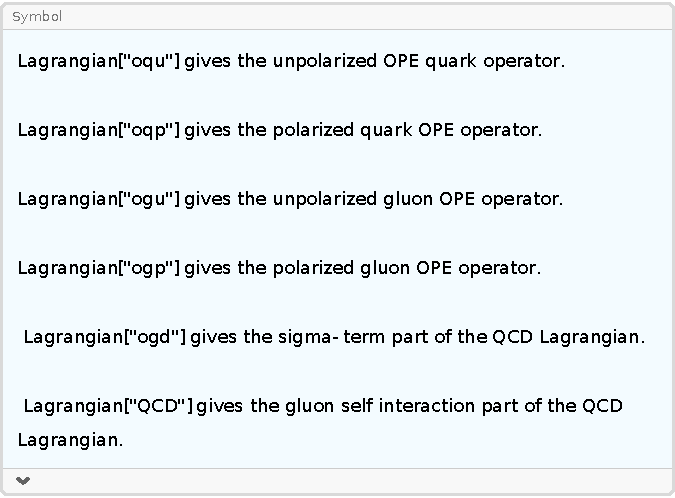
\includegraphics[width=0.6\linewidth]{img/1q4w0yoqha2oe.pdf}
\end{figure}
\FloatBarrier

\(\phi ^4\) Feynman rule

\begin{Shaded}
\begin{Highlighting}[]
\SpecialCharTok{{-}} \SpecialCharTok{\textbackslash{}}\OperatorTok{[}\NormalTok{Lambda}\OperatorTok{]}\SpecialCharTok{/}\DecValTok{4}\NormalTok{! QuantumField}\OperatorTok{[}\SpecialCharTok{\textbackslash{}}\OperatorTok{[}\NormalTok{Phi}\OperatorTok{]]}\SpecialCharTok{\^{}}\DecValTok{4} 
 
\NormalTok{FeynRule}\OperatorTok{[}\SpecialCharTok{\%}\OperatorTok{,} \OperatorTok{\{}\NormalTok{QuantumField}\OperatorTok{[}\SpecialCharTok{\textbackslash{}}\OperatorTok{[}\NormalTok{Phi}\OperatorTok{]][}\NormalTok{p1}\OperatorTok{],}\NormalTok{ QuantumField}\OperatorTok{[}\SpecialCharTok{\textbackslash{}}\OperatorTok{[}\NormalTok{Phi}\OperatorTok{]][}\NormalTok{p2}\OperatorTok{],} 
\NormalTok{   QuantumField}\OperatorTok{[}\SpecialCharTok{\textbackslash{}}\OperatorTok{[}\NormalTok{Phi}\OperatorTok{]][}\NormalTok{p3}\OperatorTok{],}\NormalTok{ QuantumField}\OperatorTok{[}\SpecialCharTok{\textbackslash{}}\OperatorTok{[}\NormalTok{Phi}\OperatorTok{]][}\NormalTok{p4}\OperatorTok{]\}]}
\end{Highlighting}
\end{Shaded}

\begin{dmath*}\breakingcomma
-\frac{\lambda  \phi ^4}{24}
\end{dmath*}

\begin{dmath*}\breakingcomma
-i \lambda
\end{dmath*}

Quark-gluon vertex Feynman rule

\begin{Shaded}
\begin{Highlighting}[]
\FunctionTok{I}\NormalTok{ QuantumField}\OperatorTok{[}\NormalTok{AntiQuarkField}\OperatorTok{]}\NormalTok{ . GA}\OperatorTok{[}\SpecialCharTok{\textbackslash{}}\OperatorTok{[}\NormalTok{Mu}\OperatorTok{]]}\NormalTok{ . CovariantD}\OperatorTok{[}\SpecialCharTok{\textbackslash{}}\OperatorTok{[}\NormalTok{Mu}\OperatorTok{]]}\NormalTok{ . QuantumField}\OperatorTok{[}\NormalTok{QuarkField}\OperatorTok{]} 
 
\NormalTok{FeynRule}\OperatorTok{[}\SpecialCharTok{\%}\OperatorTok{,} \OperatorTok{\{}\NormalTok{QuantumField}\OperatorTok{[}\NormalTok{GaugeField}\OperatorTok{,} \OperatorTok{\{}\SpecialCharTok{\textbackslash{}}\OperatorTok{[}\NormalTok{Mu}\OperatorTok{]\},} \OperatorTok{\{}\FunctionTok{a}\OperatorTok{\}][}\NormalTok{p1}\OperatorTok{],} 
\NormalTok{   QuantumField}\OperatorTok{[}\NormalTok{QuarkField}\OperatorTok{][}\NormalTok{p2}\OperatorTok{],}\NormalTok{ QuantumField}\OperatorTok{[}\NormalTok{AntiQuarkField}\OperatorTok{][}\NormalTok{p3}\OperatorTok{]\}]}
\end{Highlighting}
\end{Shaded}

\begin{dmath*}\breakingcomma
i \bar{\psi }.\bar{\gamma }^{\mu }.D_{\mu }.\psi
\end{dmath*}

\begin{dmath*}\breakingcomma
i T^a g_s \bar{\gamma }^{\mu }
\end{dmath*}

4-gluon vertex Feynman rule

\begin{Shaded}
\begin{Highlighting}[]
\SpecialCharTok{{-}}\NormalTok{(}\DecValTok{1}\SpecialCharTok{/}\DecValTok{4}\NormalTok{) FieldStrength}\OperatorTok{[}\SpecialCharTok{\textbackslash{}}\OperatorTok{[}\NormalTok{Alpha}\OperatorTok{],} \SpecialCharTok{\textbackslash{}}\OperatorTok{[}\FunctionTok{Beta}\OperatorTok{],} \FunctionTok{i}\OperatorTok{]}\NormalTok{ . FieldStrength}\OperatorTok{[}\SpecialCharTok{\textbackslash{}}\OperatorTok{[}\NormalTok{Alpha}\OperatorTok{],} \SpecialCharTok{\textbackslash{}}\OperatorTok{[}\FunctionTok{Beta}\OperatorTok{],} \FunctionTok{i}\OperatorTok{]} 
 
\NormalTok{FeynRule}\OperatorTok{[}\SpecialCharTok{\%}\OperatorTok{,} \OperatorTok{\{}\NormalTok{QuantumField}\OperatorTok{[}\NormalTok{GaugeField}\OperatorTok{,} \OperatorTok{\{}\SpecialCharTok{\textbackslash{}}\OperatorTok{[}\NormalTok{Mu}\OperatorTok{]\},} \OperatorTok{\{}\FunctionTok{a}\OperatorTok{\}][}\NormalTok{p1}\OperatorTok{],}\NormalTok{ QuantumField}\OperatorTok{[}\NormalTok{GaugeField}\OperatorTok{,} \OperatorTok{\{}\SpecialCharTok{\textbackslash{}}\OperatorTok{[}\NormalTok{Nu}\OperatorTok{]\},} \OperatorTok{\{}\FunctionTok{b}\OperatorTok{\}][}\NormalTok{p2}\OperatorTok{],} 
\NormalTok{    QuantumField}\OperatorTok{[}\NormalTok{GaugeField}\OperatorTok{,} \OperatorTok{\{}\SpecialCharTok{\textbackslash{}}\OperatorTok{[}\NormalTok{Rho}\OperatorTok{]\},} \OperatorTok{\{}\FunctionTok{c}\OperatorTok{\}][}\NormalTok{p3}\OperatorTok{],}\NormalTok{ QuantumField}\OperatorTok{[}\NormalTok{GaugeField}\OperatorTok{,} \OperatorTok{\{}\SpecialCharTok{\textbackslash{}}\OperatorTok{[}\NormalTok{Sigma}\OperatorTok{]\},} \OperatorTok{\{}\FunctionTok{d}\OperatorTok{\}][}\NormalTok{p4}\OperatorTok{]\}]} 
 
\NormalTok{GluonVertex}\OperatorTok{[\{}\FunctionTok{p}\OperatorTok{,} \SpecialCharTok{\textbackslash{}}\OperatorTok{[}\NormalTok{Mu}\OperatorTok{],} \FunctionTok{a}\OperatorTok{\},} \OperatorTok{\{}\FunctionTok{q}\OperatorTok{,} \SpecialCharTok{\textbackslash{}}\OperatorTok{[}\NormalTok{Nu}\OperatorTok{],} \FunctionTok{b}\OperatorTok{\},} \OperatorTok{\{}\FunctionTok{r}\OperatorTok{,} \SpecialCharTok{\textbackslash{}}\OperatorTok{[}\NormalTok{Rho}\OperatorTok{],} \FunctionTok{c}\OperatorTok{\},} \OperatorTok{\{}\FunctionTok{s}\OperatorTok{,} \SpecialCharTok{\textbackslash{}}\OperatorTok{[}\NormalTok{Sigma}\OperatorTok{],} \FunctionTok{d}\OperatorTok{\},}\NormalTok{ Dimension }\OtherTok{{-}\textgreater{}} \DecValTok{4}\OperatorTok{,}\NormalTok{ Explicit }\OtherTok{{-}\textgreater{}} \ConstantTok{True}\OperatorTok{]} 
 
\NormalTok{FCCanonicalizeDummyIndices}\OperatorTok{[}\SpecialCharTok{\%} \SpecialCharTok{{-}} \SpecialCharTok{\%\%}\OperatorTok{]} \SpecialCharTok{//} \FunctionTok{Factor}
\end{Highlighting}
\end{Shaded}

\begin{dmath*}\breakingcomma
-\frac{1}{4} F_{\alpha \beta }^i.F_{\alpha \beta }^i
\end{dmath*}

\begin{dmath*}\breakingcomma
i g_s^2 f^{ad\text{FCGV}(\text{si46})} f^{bc\text{FCGV}(\text{si46})} \left(\bar{g}^{\mu \rho } \bar{g}^{\nu \sigma }-\bar{g}^{\mu \nu } \bar{g}^{\rho \sigma }\right)+i g_s^2 f^{ac\text{FCGV}(\text{si46})} f^{bd\text{FCGV}(\text{si46})} \left(\bar{g}^{\mu \sigma } \bar{g}^{\nu \rho }-\bar{g}^{\mu \nu } \bar{g}^{\rho \sigma }\right)+i g_s^2 f^{ab\text{FCGV}(\text{si46})} f^{cd\text{FCGV}(\text{si46})} \left(\bar{g}^{\mu \sigma } \bar{g}^{\nu \rho }-\bar{g}^{\mu \rho } \bar{g}^{\nu \sigma }\right)
\end{dmath*}

\begin{dmath*}\breakingcomma
-i g_s^2 \left(f^{ad\text{FCGV}(\text{u53})} f^{bc\text{FCGV}(\text{u53})} \left(\bar{g}^{\mu \nu } \bar{g}^{\rho \sigma }-\bar{g}^{\mu \rho } \bar{g}^{\nu \sigma }\right)+f^{ac\text{FCGV}(\text{u53})} f^{bd\text{FCGV}(\text{u53})} \left(\bar{g}^{\mu \nu } \bar{g}^{\rho \sigma }-\bar{g}^{\mu \sigma } \bar{g}^{\nu \rho }\right)+f^{ab\text{FCGV}(\text{u53})} f^{cd\text{FCGV}(\text{u53})} \left(\bar{g}^{\mu \rho } \bar{g}^{\nu \sigma }-\bar{g}^{\mu \sigma } \bar{g}^{\nu \rho }\right)\right)
\end{dmath*}

\begin{dmath*}\breakingcomma
0
\end{dmath*}

3-gluon vertex Feynman rule

\begin{Shaded}
\begin{Highlighting}[]
\SpecialCharTok{{-}}\NormalTok{(}\DecValTok{1}\SpecialCharTok{/}\DecValTok{4}\NormalTok{) FieldStrength}\OperatorTok{[}\SpecialCharTok{\textbackslash{}}\OperatorTok{[}\NormalTok{Alpha}\OperatorTok{],} \SpecialCharTok{\textbackslash{}}\OperatorTok{[}\FunctionTok{Beta}\OperatorTok{],} \FunctionTok{i}\OperatorTok{]}\NormalTok{ . FieldStrength}\OperatorTok{[}\SpecialCharTok{\textbackslash{}}\OperatorTok{[}\NormalTok{Alpha}\OperatorTok{],} \SpecialCharTok{\textbackslash{}}\OperatorTok{[}\FunctionTok{Beta}\OperatorTok{],} \FunctionTok{i}\OperatorTok{]} 
 
\NormalTok{FeynRule}\OperatorTok{[}\SpecialCharTok{\%}\OperatorTok{,} \OperatorTok{\{}\NormalTok{QuantumField}\OperatorTok{[}\NormalTok{GaugeField}\OperatorTok{,} \OperatorTok{\{}\SpecialCharTok{\textbackslash{}}\OperatorTok{[}\NormalTok{Mu}\OperatorTok{]\},} \OperatorTok{\{}\FunctionTok{a}\OperatorTok{\}][}\FunctionTok{p}\OperatorTok{],}\NormalTok{ QuantumField}\OperatorTok{[}\NormalTok{GaugeField}\OperatorTok{,} \OperatorTok{\{}\SpecialCharTok{\textbackslash{}}\OperatorTok{[}\NormalTok{Nu}\OperatorTok{]\},} \OperatorTok{\{}\FunctionTok{b}\OperatorTok{\}][}\FunctionTok{q}\OperatorTok{],} 
\NormalTok{    QuantumField}\OperatorTok{[}\NormalTok{GaugeField}\OperatorTok{,} \OperatorTok{\{}\SpecialCharTok{\textbackslash{}}\OperatorTok{[}\NormalTok{Rho}\OperatorTok{]\},} \OperatorTok{\{}\FunctionTok{c}\OperatorTok{\}][}\FunctionTok{r}\OperatorTok{]\}]} 
 
\NormalTok{GluonVertex}\OperatorTok{[\{}\FunctionTok{p}\OperatorTok{,} \SpecialCharTok{\textbackslash{}}\OperatorTok{[}\NormalTok{Mu}\OperatorTok{],} \FunctionTok{a}\OperatorTok{\},} \OperatorTok{\{}\FunctionTok{q}\OperatorTok{,} \SpecialCharTok{\textbackslash{}}\OperatorTok{[}\NormalTok{Nu}\OperatorTok{],} \FunctionTok{b}\OperatorTok{\},} \OperatorTok{\{}\FunctionTok{r}\OperatorTok{,} \SpecialCharTok{\textbackslash{}}\OperatorTok{[}\NormalTok{Rho}\OperatorTok{],} \FunctionTok{c}\OperatorTok{\},}\NormalTok{ Dimension }\OtherTok{{-}\textgreater{}} \DecValTok{4}\OperatorTok{,}\NormalTok{ Explicit }\OtherTok{{-}\textgreater{}} \ConstantTok{True}\OperatorTok{]} 
 
\NormalTok{ExpandScalarProduct}\OperatorTok{[}\SpecialCharTok{\%} \SpecialCharTok{{-}} \SpecialCharTok{\%\%}\OperatorTok{]} \SpecialCharTok{//} \FunctionTok{Factor}
\end{Highlighting}
\end{Shaded}

\begin{dmath*}\breakingcomma
-\frac{1}{4} F_{\alpha \beta }^i.F_{\alpha \beta }^i
\end{dmath*}

\begin{dmath*}\breakingcomma
g_s f^{abc} \left(\bar{g}^{\mu \nu } \left(\overline{p}^{\rho }-\overline{q}^{\rho }\right)-\bar{g}^{\mu \rho } \left(\overline{p}^{\nu }-\overline{r}^{\nu }\right)+\bar{g}^{\nu \rho } \left(\overline{q}^{\mu }-\overline{r}^{\mu }\right)\right)
\end{dmath*}

\begin{dmath*}\breakingcomma
g_s f^{abc} \left(\bar{g}^{\mu \nu } \left(\overline{p}-\overline{q}\right)^{\rho }+\bar{g}^{\mu \rho } \left(\overline{r}-\overline{p}\right)^{\nu }+\bar{g}^{\nu \rho } \left(\overline{q}-\overline{r}\right)^{\mu }\right)
\end{dmath*}

\begin{dmath*}\breakingcomma
0
\end{dmath*}

Higgs EFT interaction vertex

\begin{Shaded}
\begin{Highlighting}[]
\NormalTok{heftInt }\ExtensionTok{=} \SpecialCharTok{{-}}\NormalTok{(}\DecValTok{1}\SpecialCharTok{/}\DecValTok{4}\NormalTok{) CH FieldStrength}\OperatorTok{[}\NormalTok{mu}\OperatorTok{,}\NormalTok{ nu}\OperatorTok{,} \FunctionTok{a}\OperatorTok{]}\NormalTok{ . FieldStrength}\OperatorTok{[}\NormalTok{mu}\OperatorTok{,}\NormalTok{ nu}\OperatorTok{,} \FunctionTok{a}\OperatorTok{]}\NormalTok{ . QuantumField}\OperatorTok{[}\FunctionTok{H}\OperatorTok{]}
\end{Highlighting}
\end{Shaded}

\begin{dmath*}\breakingcomma
-\frac{1}{4} \;\text{CH} F_{\text{mu}\;\text{nu}}^a.F_{\text{mu}\;\text{nu}}^a.H
\end{dmath*}

\(Hgg\) vertex Feynman rules

\begin{Shaded}
\begin{Highlighting}[]
\NormalTok{FeynRule}\OperatorTok{[}\NormalTok{heftInt}\OperatorTok{,} \OperatorTok{\{}\NormalTok{QuantumField}\OperatorTok{[}\NormalTok{GaugeField}\OperatorTok{,} \OperatorTok{\{}\FunctionTok{i}\OperatorTok{\},} \OperatorTok{\{}\FunctionTok{a}\OperatorTok{\}][}\NormalTok{p1}\OperatorTok{],}\NormalTok{ QuantumField}\OperatorTok{[}\NormalTok{GaugeField}\OperatorTok{,} 
     \OperatorTok{\{}\FunctionTok{j}\OperatorTok{\},} \OperatorTok{\{}\FunctionTok{b}\OperatorTok{\}][}\NormalTok{p2}\OperatorTok{],}\NormalTok{ QuantumField}\OperatorTok{[}\FunctionTok{H}\OperatorTok{][}\NormalTok{p3}\OperatorTok{]\}]}
\end{Highlighting}
\end{Shaded}

\begin{dmath*}\breakingcomma
-i \;\text{CH} \delta ^{ab} \left(\overline{\text{p2}}^i \overline{\text{p1}}^j-\bar{g}^{ij} \left(\overline{\text{p1}}\cdot \overline{\text{p2}}\right)\right)
\end{dmath*}

\(Hggg\) vertex Feynman rules

\begin{Shaded}
\begin{Highlighting}[]
\NormalTok{FeynRule}\OperatorTok{[}\NormalTok{heftInt}\OperatorTok{,} \OperatorTok{\{}\NormalTok{QuantumField}\OperatorTok{[}\NormalTok{GaugeField}\OperatorTok{,} \OperatorTok{\{}\FunctionTok{i}\OperatorTok{\},} \OperatorTok{\{}\FunctionTok{a}\OperatorTok{\}][}\NormalTok{p1}\OperatorTok{],}\NormalTok{ QuantumField}\OperatorTok{[}\NormalTok{GaugeField}\OperatorTok{,} 
      \OperatorTok{\{}\FunctionTok{j}\OperatorTok{\},} \OperatorTok{\{}\FunctionTok{b}\OperatorTok{\}][}\NormalTok{p2}\OperatorTok{],}\NormalTok{ QuantumField}\OperatorTok{[}\NormalTok{GaugeField}\OperatorTok{,} \OperatorTok{\{}\FunctionTok{k}\OperatorTok{\},} \OperatorTok{\{}\FunctionTok{c}\OperatorTok{\}][}\NormalTok{p3}\OperatorTok{],}\NormalTok{ QuantumField}\OperatorTok{[}\FunctionTok{H}\OperatorTok{][}\NormalTok{p4}\OperatorTok{]\}]} \SpecialCharTok{//} \FunctionTok{Simplify}
\end{Highlighting}
\end{Shaded}

\begin{dmath*}\breakingcomma
\text{CH} g_s f^{abc} \left(\bar{g}^{ij} \left(\overline{\text{p1}}^k-\overline{\text{p2}}^k\right)-\bar{g}^{ik} \left(\overline{\text{p1}}^j-\overline{\text{p3}}^j\right)+\bar{g}^{jk} \left(\overline{\text{p2}}^i-\overline{\text{p3}}^i\right)\right)
\end{dmath*}

\(Hgggg\) vertex Feynman rules

\begin{Shaded}
\begin{Highlighting}[]
\NormalTok{FeynRule}\OperatorTok{[}\NormalTok{heftInt}\OperatorTok{,} \OperatorTok{\{}\NormalTok{QuantumField}\OperatorTok{[}\NormalTok{GaugeField}\OperatorTok{,} \OperatorTok{\{}\FunctionTok{i}\OperatorTok{\},} \OperatorTok{\{}\FunctionTok{a}\OperatorTok{\}][}\NormalTok{p1}\OperatorTok{],}\NormalTok{ QuantumField}\OperatorTok{[}\NormalTok{GaugeField}\OperatorTok{,} \OperatorTok{\{}\FunctionTok{j}\OperatorTok{\},} 
       \OperatorTok{\{}\FunctionTok{b}\OperatorTok{\}][}\NormalTok{p2}\OperatorTok{],}\NormalTok{ QuantumField}\OperatorTok{[}\NormalTok{GaugeField}\OperatorTok{,} \OperatorTok{\{}\FunctionTok{k}\OperatorTok{\},} \OperatorTok{\{}\FunctionTok{c}\OperatorTok{\}][}\NormalTok{p3}\OperatorTok{],} 
\NormalTok{     QuantumField}\OperatorTok{[}\NormalTok{GaugeField}\OperatorTok{,} \OperatorTok{\{}\FunctionTok{l}\OperatorTok{\},} \OperatorTok{\{}\FunctionTok{d}\OperatorTok{\}][}\NormalTok{p4}\OperatorTok{],}\NormalTok{ QuantumField}\OperatorTok{[}\FunctionTok{H}\OperatorTok{][}\NormalTok{p5}\OperatorTok{]\}]} \SpecialCharTok{//} 
\NormalTok{   FCCanonicalizeDummyIndices}\OperatorTok{[}\NormalTok{\#}\OperatorTok{,}\NormalTok{ SUNIndexNames }\OtherTok{{-}\textgreater{}} \OperatorTok{\{}\FunctionTok{e}\OperatorTok{\}]}\NormalTok{ \& }\SpecialCharTok{//}\NormalTok{ Collect2}\OperatorTok{[}\NormalTok{\#}\OperatorTok{,}\NormalTok{ SUNF}\OperatorTok{,} 
\NormalTok{    FCFactorOut }\OtherTok{{-}\textgreater{}} \FunctionTok{I}\NormalTok{ CH SMP}\OperatorTok{[}\StringTok{"g\_s"}\OperatorTok{]}\SpecialCharTok{\^{}}\DecValTok{2}\OperatorTok{]}\NormalTok{ \&}
\end{Highlighting}
\end{Shaded}

\begin{dmath*}\breakingcomma
i \;\text{CH} g_s^2 \left(f^{ade} f^{bce} \left(\bar{g}^{ik} \bar{g}^{jl}-\bar{g}^{ij} \bar{g}^{kl}\right)+f^{ace} f^{bde} \left(\bar{g}^{il} \bar{g}^{jk}-\bar{g}^{ij} \bar{g}^{kl}\right)+f^{abe} f^{cde} \left(\bar{g}^{il} \bar{g}^{jk}-\bar{g}^{ik} \bar{g}^{jl}\right)\right)
\end{dmath*}

Some OPE-related examples:

2-gluon Feynman rules (unpolarized).

\begin{Shaded}
\begin{Highlighting}[]
\NormalTok{Lagrangian}\OperatorTok{[}\StringTok{"ogu"}\OperatorTok{]}
\NormalTok{FeynRule}\OperatorTok{[}\SpecialCharTok{\%}\OperatorTok{,} \OperatorTok{\{}\NormalTok{QuantumField}\OperatorTok{[}\NormalTok{GaugeField}\OperatorTok{,} \OperatorTok{\{}\SpecialCharTok{\textbackslash{}}\OperatorTok{[}\NormalTok{Mu}\OperatorTok{]\},} \OperatorTok{\{}\FunctionTok{a}\OperatorTok{\}][}\FunctionTok{p}\OperatorTok{],}\NormalTok{ QuantumField}\OperatorTok{[}\NormalTok{GaugeField}\OperatorTok{,} \OperatorTok{\{}\SpecialCharTok{\textbackslash{}}\OperatorTok{[}\NormalTok{Nu}\OperatorTok{]\},} 
      \OperatorTok{\{}\FunctionTok{b}\OperatorTok{\}][}\FunctionTok{q}\OperatorTok{]\},}\NormalTok{ ZeroMomentumInsertion }\OtherTok{{-}\textgreater{}} \ConstantTok{False}\OperatorTok{]} \SpecialCharTok{//} \FunctionTok{Factor}
\end{Highlighting}
\end{Shaded}

\begin{dmath*}\breakingcomma
\frac{1}{2} i^{m-1} F_{\text{FCGV}(\alpha )\Delta }^{\text{FCGV}(\text{a})}.\left(D_{\Delta }^{\text{FCGV}(\text{a})\text{FCGV}(\text{b})}\right){}^{m-2}.F_{\text{FCGV}(\alpha )\Delta }^{\text{FCGV}(\text{b})}
\end{dmath*}

\begin{dmath*}\breakingcomma
-i^m \delta ^{ab} \left(\vec{\partial }_{\Delta }\right){}^{m-2} \left(-\bar{g}^{\mu \nu } \left(\Delta \cdot \overline{p}\right) \left(\Delta \cdot \overline{q}\right)+\Delta ^{\nu } \overline{q}^{\mu } \left(\Delta \cdot \overline{p}\right)+\Delta ^{\mu } \overline{p}^{\nu } \left(\Delta \cdot \overline{q}\right)-\Delta ^{\mu } \Delta ^{\nu } \left(\overline{p}\cdot \overline{q}\right)\right)
\end{dmath*}

2-gluon Feynman rules (polarized).

\begin{Shaded}
\begin{Highlighting}[]
\NormalTok{Lagrangian}\OperatorTok{[}\StringTok{"ogp"}\OperatorTok{]}
\NormalTok{FeynRule}\OperatorTok{[}\SpecialCharTok{\%}\OperatorTok{,} \OperatorTok{\{}\NormalTok{QuantumField}\OperatorTok{[}\NormalTok{GaugeField}\OperatorTok{,} \OperatorTok{\{}\SpecialCharTok{\textbackslash{}}\OperatorTok{[}\NormalTok{Mu}\OperatorTok{]\},} \OperatorTok{\{}\FunctionTok{a}\OperatorTok{\}][}\FunctionTok{p}\OperatorTok{],}\NormalTok{ QuantumField}\OperatorTok{[}\NormalTok{GaugeField}\OperatorTok{,} \OperatorTok{\{}\SpecialCharTok{\textbackslash{}}\OperatorTok{[}\NormalTok{Nu}\OperatorTok{]\},} 
       \OperatorTok{\{}\FunctionTok{b}\OperatorTok{\}][}\FunctionTok{q}\OperatorTok{]\},}\NormalTok{ ZeroMomentumInsertion }\OtherTok{{-}\textgreater{}} \ConstantTok{False}\OperatorTok{]} \SpecialCharTok{//} \FunctionTok{Factor} 
 
\NormalTok{Factor2}\OperatorTok{[}\NormalTok{Calc}\OperatorTok{[}\SpecialCharTok{\%} \OtherTok{/.} \FunctionTok{p} \OtherTok{{-}\textgreater{}} \SpecialCharTok{{-}}\FunctionTok{q}\OperatorTok{,} \FunctionTok{Assumptions} \OtherTok{{-}\textgreater{}} \ConstantTok{Automatic}\OperatorTok{]]}
\end{Highlighting}
\end{Shaded}

\begin{dmath*}\breakingcomma
\frac{1}{2} i^m \bar{\epsilon }^{\text{FCGV}(\alpha )\text{FCGV}(\beta )\text{FCGV}(\gamma )\Delta }.F_{\text{FCGV}(\beta )\text{FCGV}(\gamma )}^{\text{FCGV}(\text{a})}.\left(D_{\Delta }^{\text{FCGV}(\text{a})\text{FCGV}(\text{b})}\right){}^{m-2}.F_{\text{FCGV}(\alpha )\Delta }^{\text{FCGV}(\text{b})}
\end{dmath*}

\begin{dmath*}\breakingcomma
0
\end{dmath*}

\begin{dmath*}\breakingcomma
0
\end{dmath*}

Compare with the Feynman rule tabulated in Twist2GluonOperator.

\begin{Shaded}
\begin{Highlighting}[]
\NormalTok{Twist2GluonOperator}\OperatorTok{[}\FunctionTok{q}\OperatorTok{,} \OperatorTok{\{}\SpecialCharTok{\textbackslash{}}\OperatorTok{[}\NormalTok{Mu}\OperatorTok{],} \FunctionTok{a}\OperatorTok{\},} \OperatorTok{\{}\SpecialCharTok{\textbackslash{}}\OperatorTok{[}\NormalTok{Nu}\OperatorTok{],} \FunctionTok{b}\OperatorTok{\},}\NormalTok{ Polarization }\OtherTok{{-}\textgreater{}} \DecValTok{1}\OperatorTok{,}\NormalTok{ Explicit }\OtherTok{{-}\textgreater{}} \ConstantTok{True}\OperatorTok{]}
\end{Highlighting}
\end{Shaded}

\begin{dmath*}\breakingcomma
i \left(1-(-1)^m\right) \delta ^{ab} (\Delta \cdot q)^{m-1} \overset{\text{}}{\epsilon }^{\mu \nu \Delta q}
\end{dmath*}

quark-quark -gluon-gluon Feynman rule (unpolarized).

\begin{Shaded}
\begin{Highlighting}[]
\NormalTok{Lagrangian}\OperatorTok{[}\StringTok{"oqu"}\OperatorTok{]} 
 
\NormalTok{frule }\ExtensionTok{=}\NormalTok{ FeynRule}\OperatorTok{[}\SpecialCharTok{\%}\OperatorTok{,} \OperatorTok{\{}\NormalTok{QuantumField}\OperatorTok{[}\NormalTok{QuarkField}\OperatorTok{][}\FunctionTok{p}\OperatorTok{],}\NormalTok{ QuantumField}\OperatorTok{[}\NormalTok{AntiQuarkField}\OperatorTok{][}\FunctionTok{q}\OperatorTok{],} 
\NormalTok{     QuantumField}\OperatorTok{[}\NormalTok{GaugeField}\OperatorTok{,} \OperatorTok{\{}\SpecialCharTok{\textbackslash{}}\OperatorTok{[}\NormalTok{Mu}\OperatorTok{]\},} \OperatorTok{\{}\FunctionTok{a}\OperatorTok{\}][}\FunctionTok{r}\OperatorTok{],}\NormalTok{ QuantumField}\OperatorTok{[}\NormalTok{GaugeField}\OperatorTok{,} \OperatorTok{\{}\SpecialCharTok{\textbackslash{}}\OperatorTok{[}\NormalTok{Nu}\OperatorTok{]\},} \OperatorTok{\{}\FunctionTok{b}\OperatorTok{\}][}\FunctionTok{s}\OperatorTok{]\},} 
\NormalTok{    ZeroMomentumInsertion }\OtherTok{{-}\textgreater{}} \ConstantTok{True}\OperatorTok{,}\NormalTok{ InitialFunction }\OtherTok{{-}\textgreater{}} \FunctionTok{Identity}\OperatorTok{]}\NormalTok{;}
\end{Highlighting}
\end{Shaded}

\begin{dmath*}\breakingcomma
i^m \bar{\psi }.\left(\bar{\gamma }\cdot \Delta \right).D_{\Delta }{}^{m-1}.\psi
\end{dmath*}

\begin{Shaded}
\begin{Highlighting}[]
\FunctionTok{LeafCount}\OperatorTok{[}\NormalTok{frule}\OperatorTok{]}
\end{Highlighting}
\end{Shaded}

\begin{dmath*}\breakingcomma
39364
\end{dmath*}

\begin{Shaded}
\begin{Highlighting}[]
\NormalTok{Twist2QuarkOperator}\OperatorTok{[\{}\FunctionTok{p}\OperatorTok{\},} \OperatorTok{\{}\FunctionTok{q}\OperatorTok{\},} \OperatorTok{\{}\FunctionTok{r}\OperatorTok{,} \SpecialCharTok{\textbackslash{}}\OperatorTok{[}\NormalTok{Mu}\OperatorTok{],} \FunctionTok{a}\OperatorTok{\},} \OperatorTok{\{}\FunctionTok{s}\OperatorTok{,} \SpecialCharTok{\textbackslash{}}\OperatorTok{[}\NormalTok{Nu}\OperatorTok{],} \FunctionTok{b}\OperatorTok{\},}\NormalTok{ Polarization }\OtherTok{{-}\textgreater{}} \DecValTok{0}\OperatorTok{]}
\end{Highlighting}
\end{Shaded}

\begin{dmath*}\breakingcomma
-(-1)^m \Delta ^{\mu } \Delta ^{\nu } g_s^2 \left(\bar{\gamma }\cdot \Delta \right).\left(T^a.T^b \left(\sum _{i=0}^{-3+m} \;\text{}\;\text{} (i+1)(\Delta \cdot q)^j (-(\Delta \cdot p))^{-i+m-3} (\Delta \cdot q+\Delta \cdot r)^{i-j}\right)+T^b.T^a \left(\sum _{i=0}^{-3+m} \;\text{}\;\text{} (i+1)(\Delta \cdot q)^j (-(\Delta \cdot p))^{-i+m-3} (\Delta \cdot q+\Delta \cdot s)^{i-j}\right)\right)
\end{dmath*}

\begin{Shaded}
\begin{Highlighting}[]
\CommentTok{(*Twist2QuarkOperator[\{p\},\{q\},\{r,\textbackslash{}[Mu],a\},\{s,\textbackslash{}[Nu],b\},Polarization{-}\textgreater{}0]}
\CommentTok{Calc[frule{-}\%\%/.OPEm{-}\textgreater{}5/.s{-}\textgreater{}{-}p{-}q{-}r/.D{-}\textgreater{}4]*)}
\end{Highlighting}
\end{Shaded}

\end{document}
